\documentclass{article}


% if you need to pass options to natbib, use, e.g.:
%     \PassOptionsToPackage{numbers, compress}{natbib}
% before loading neurips_2024


% ready for submission
% \usepackage{neurips_2024}


% to compile a preprint version, e.g., for submission to arXiv, add add the
% [preprint] option:
%     \usepackage[preprint]{neurips_2024}


% to compile a camera-ready version, add the [final] option, e.g.:
    \usepackage[final]{neurips_2024}


% to avoid loading the natbib package, add option nonatbib:
%    \usepackage[nonatbib]{neurips_2024}

\usepackage{natbib}
\usepackage[utf8]{inputenc} % allow utf-8 input
\usepackage[T1]{fontenc}    % use 8-bit T1 fonts
\usepackage{hyperref}       % hyperlinks
\usepackage{url}            % simple URL typesetting
\usepackage{booktabs}       % professional-quality tables
\usepackage{amsfonts}       % blackboard math symbols
\usepackage{nicefrac}       % compact symbols for 1/2, etc.
\usepackage{microtype}      % microtypography
\usepackage{xcolor}         % colors
\usepackage{amsmath}
\usepackage{amssymb}
\usepackage{graphicx}

\newcommand{\bfx}{\textbf{x}}
\DeclareMathOperator*{\argmin}{arg\,min}

\title{Non-Myopic Bayesian Optimization with Unknown Cost Constraints}


% The \author macro works with any number of authors. There are two commands
% used to separate the names and addresses of multiple authors: \And and \AND.
%
% Using \And between authors leaves it to LaTeX to determine where to break the
% lines. Using \AND forces a line break at that point. So, if LaTeX puts 3 of 4
% authors names on the first line, and the last on the second line, try using
% \AND instead of \And before the third author name.


\author{%
  Ethan Hersch$^*$ \\
  Department of Computer Science\\
  Cornell University\\
  Ithaca, NY 14853 \\
  \texttt{esh87@cornell.edu} \\
  % examples of more authors
  \And
  Mohammad Islam$^*$ \\
  Department of Computer Science\\
  Cornell University\\
  Ithaca, NY 14853 \\
  \texttt{mai54@cornell.edu} \\
  \And
  Darian Nwankwo$^*$ \\
  Department of Computer Science\\
  Cornell University\\
  Ithaca, NY 14853 \\
  \texttt{don4@cornell.edu} \\
  \And
  Shahrukh Showkath$^*$ \\
  Department of Computer Science\\
  Cornell University\\
  Ithaca, NY 14853 \\
  \texttt{ss4266@cornell.edu} \\
  % \AND
  % Coauthor \\
  % Affiliation \\
  % Address \\
  % \texttt{email} \\
  % \And
  % Coauthor \\
  % Affiliation \\
  % Address \\
  % \texttt{email} \\
  % \And
  % Coauthor \\
  % Affiliation \\
  % Address \\
  % \texttt{email} \\
}


\begin{document}


\maketitle
\def\thefootnote{*}\footnotetext{These authors contributed equally to this work}\def\thefootnote{\arabic{footnote}}


\begin{abstract}
  Bayesian Optimization (BO) is a powerful tool for optimizing 
  expensive black-box functions. It treats the objective function 
  as a probabilistic model and iteratively updates this model 
  based on observations, typically using Gaussian Processes (GPs). 
  Bayesian optimization can be used in a setting where evaluation 
  is expensive, say tuning the parameters of a neural network to 
  optimize accuracy. Consider the scenario where each evaluation 
  point has a cost associated to it, and there is a budget of the 
  total cost to optimize the underlying function. Say this cost is 
  unknown a-priori and it must be explored as the objective 
  function is evaluated. This is the setting this paper will 
  explore and propose a methodology to model such a scenario by 
  building a GP around both the cost function and objective 
  function.
\end{abstract}


\section{Introduction}
Bayesian optimization (BO) algorithms are sample-efficient methods for global optimization of
expensive continuous ``black-box'' functions where derivative 
information isn't available. We assume these functions are 
defined over a compact set where evaluation is expensive. BO 
builds a statistical model of the objective function based on 
samples. BO further builds an acquisition function, conditioned on the statistical model, and chooses new sample locations by
optimizing this acquisition function that reflects the value of 
candidate locations.
Most BO methods use {\em myopic} acquisition functions that only 
consider the impact of the next sample where every sample has unit cost. Given the aforementioned description, our objective is the following:
\[
    x^* \in \argmin_{x \in \mathcal{X}} f(x)
\]

The de facto statisical model used in BO is a Gaussian process, 
i.e. we place a Gaussian process prior over our function
$f \sim \mathcal{GP}(m(x), k(x, x')$. A Gaussian process is a 
collection of random variables, any finite number of which
have a joint Gaussian distribution~\cite{Rasmussen2006Gaussian}.
Traditional BO methods assume the cost of evaluation is uniform
across our domain, which is implicitly encoded in most acquisition
functions. 
In practice, the cost of evaluation differs across 
our domain $\mathcal{X} \subseteq \mathbb{R}^d$ and standard
acquisition functions don't consider this. BO has established 
itself as a 
fundamental approach for optimizing complex and expensive 
functions in various domains. Its primary strength lies in its 
sample efficiency of evaluating the objective function, 
making it well-suited for applications such as hyperparameter 
tuning in neural networks.

% The expected improvement acquisition function ($EI(x)$) is a 
% common acquisition function for BO.
% \[EI(x) = (f^* - \mu(x))\Phi \left( \frac{f^* - \mu(x)}
% {\sigma(x)}\right) + \sigma(x)\phi \left(\frac{f^* - \mu(x)}
% {\sigma(x)}\right)\]
% where $f^*$ is the best point observed so far and $\mu(x)$, 
% $\sigma(x)$ are the predictive mean and variance at our point $x$. 
% $\Phi$ is the standard normal CDF and $\phi$ is the PDF. The 
% expected improvement acquisition function is powerful as it uses 
% statistics gathered on all prior observations to guide the model 
% where it has the ``best chance'' of finding a value of $f$ which is 
% higher than any previously seen.

% One can think of cost-constrained BO as the following constrained optimization problem:
% \begin{align*}
% \min_{\bfx \in \mathcal{X}} f(\bfx)
% \operatorname{subject \; to} \sum_{\bfx \in \mathcal{X}} c(\bfx)
% \leq \tau.
% \end{align*}
% We assume $f(\bfx)$ outputs not only its value, but also its evaluation cost determined by a 
% black-box cost function $c(\bfx)$. We assume the cost function has the following functional
% form: $c(\bfx) = p(\bfx) + \exp(g(\bfx))$ where $g(\bfx) \sim \mathcal{GP}(m(\bfx), k(\bfx, \bfx')$
% and $p(\bfx) = \sum_{i=0}^d a_ix^i$. That is, the cost consists of an optional deterministic 
% component plus some stochastic perturbation term that is state-independent. Our goal is to
% minimize $f(\bfx)$ subject to the total evaluation cost not exceeding $\tau$. The value of
% $\tau$ is a pre-determined upper bound on the total cost, such as compute time, dollars, or
% cloud-compute resource utilization.

% A common acquisition function for myopic cost-constrained BO is $EI$ per unit cost: 
% \[EIpu(x) = \frac{EI(x)}{c(x)}\]

% Non-myopic approaches to BO generally involve solving a dynamic 
% program to see which possible future observation could help lead 
% to the highest final prediction. But these DPs are too costly to 
% fully solve, so we must use a Markov decision process (MDP) and 
% multi-step look-ahead to infer which future observation would be 
% the best solution, globally. It is difficult to handle such 
% stochastic cost functions; to overcome this challenge we propose 
% modeling the cost as a Gaussian process as well.

\section{Background and previous work}
Traditional BO methods focus on one-step look ahead acquisition 
functions, such as Expected Improvement (EI) [A.1], which optimize 
immediate gain and do not consider future evaluations. This myopic 
approach can lead to suboptimal performance compared to a holistic 
evaluation. As a result, multi-step look-ahead acquisition functions have emerged, 
aiming to maximize the cumulative reward across multiple 
evaluations. These methods aim to balance exploration against exploitation over a finite budget. 

A prominent solution in multi step look-ahead BO formulated the 
selection process as a dynamic programming problem solved 
throughout rollout strategies \citep{lamwilcox2017}. However the computation expense of this 
rollout strategy limited the scalability of the approach. In 
response, \citep{zhang2019high}, introduced 2-OPT-C which was a 
constrained two step acquisition function utilizing likelihood 
ratios for efficient optimization and balances exploration. 
Practical advancements, such as the Monte Carlo and variance 
reduction techniques presented in the two-step look-ahead 
algorithm by Wu and Frazier have reduced this 
computational barrier making the non-myopic BO approach 
feasible in higher dimensions for larger batches~\citep{wu2019practical}. 

\citep{lee2021multistep} tackled the cost-constrained aspect of BO 
by framing it as a constrained Markov decision process (CDMP), 
where the costs are deterministic and depend on the region within the 
search space. Their approach uses a rollout approximation to the 
optimal CMDP policy by taking the cost and future iterations into 
account. This model is effective for applications where 
evaluation costs vary widely, such as hyperparameter tuning, 
where cost efficiency is more critical than sample efficiency. 

\section{Research question and approach}
Our work builds on these previous advancements by proposing a 
methodology that models the cost functions within a 
GP framework, addressing scenarios where cost functions are 
unknown and must be dynamically explored alongside the objective 
function. Simultaneously, we incorporate our stochastic model
of the cost function into the cost-constrained Markov decision
process to maintain our balance of exploration against 
exploitation. Hence, \textbf{how can we perform non-myopic cost-
constrained Bayesian optimization in a setting where the cost
function is not known ahead of time?}

One key limitation in existing non-myopic BO is the 
assumption that the cost of each evaluation is known in advance. 
This is often not the case in practice, where the cost of 
evaluation may be stochastic or unknown. The need for a cost-
aware optimization framework that can handle such scenarios is 
evident. One can think of cost-constrained BO as the following constrained optimization problem:
\begin{align*}
\min_{\bfx \in \mathcal{X}} f(\bfx)
\operatorname{subject \; to} \sum_{\bfx \in \mathcal{X}} c(\bfx)
\leq \tau.
\end{align*}
We assume $f(\bfx)$ outputs not only its value, but also its evaluation cost determined by a 
black-box cost function $c(\bfx)$. We assume the cost function has the following functional
form: $c(\bfx) = p(\bfx) + \exp(g(\bfx))$ where $g(\bfx) \sim \mathcal{GP}(m(\bfx), k(\bfx, \bfx')$
component plus some stochastic perturbation term that is state-independent. Our goal is to
minimize $f(\bfx)$ subject to the total evaluation cost not exceeding $\tau$. The value of
$\tau$ is a pre-determined upper bound on the total cost, such as compute time, dollars, or
cloud-compute resource utilization.


In such tasks, each evaluation can be 
computationally expensive, requiring a method that balances 
exploration and exploitation. BO operates effectively in 
settings where assumptions of smooth and differentiable 
objective functions do not hold, a common scenario in machine 
learning.

The classical formulation of BO typically assumes a ``myopic'' 
view of decision-making. This results in maximizing immediate 
rewards without considering the long-term consequences of the 
decision. While effective in many scenarios, this approach may 
not be optimal in settings where the cost of evaluation varies 
across the domain. This shift to non-myopic decision making 
introduces a new paradigm that extends the utility of BO.

\section{Experiments and results}

To motivate our experiments, we pick standard test optimization functions as our ``datasets'' The first notable function is the Ackley function, which is useful as it exhibits many local minima [A.2]. Other functions include the McCormick and Rosenbrock functions which exhibit a similar level of computational complexity and are selected as they have varying properties of complex optimization problems commonly found: some are bowl-shaped, plate-shaped, valley-shaped, and contain steep ridges/drops. These functions are found from Simon Fraser University: \url{https://www.sfu.ca/~ssurjano/optimization.html}. Our initial experiments deal with the Ackley function in one dimension for fast computation in testing our framework, but experiments will be extended to other functions in higher dimension.

We used BOTorch and GPyTorch to set up machinery for fitting GPs around both the cost and objective (Ackley) function. Figure 1 shows the surrogate fit around these initial samples.

\begin{figure}
    \centering
    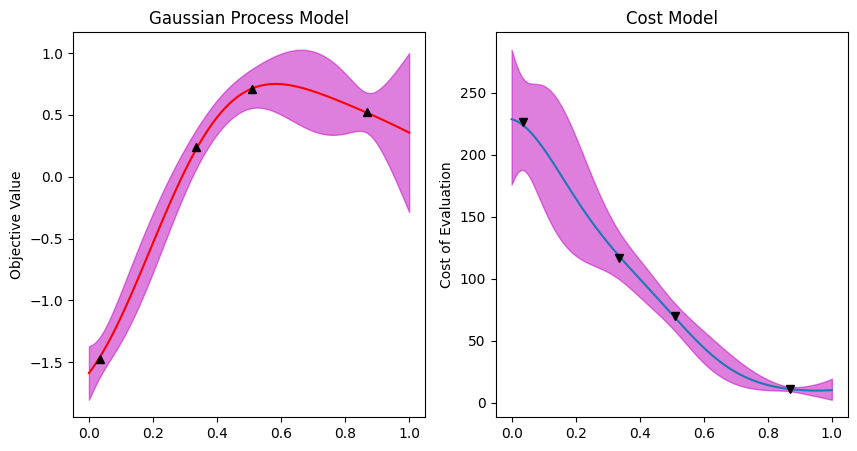
\includegraphics[width=0.7\linewidth]{graphics/gp_cost.png}
    \caption{Initial surrogate model}
\end{figure}

We then compared random sampling (a non BO technique) with the EIpu and EI acquisition functions to show how Bayesian optimization converges to a gap of 1 sooner (random sampling does not converge to a gap of 1). See figure 2 for this demonstration.

\begin{figure}
    \centering
    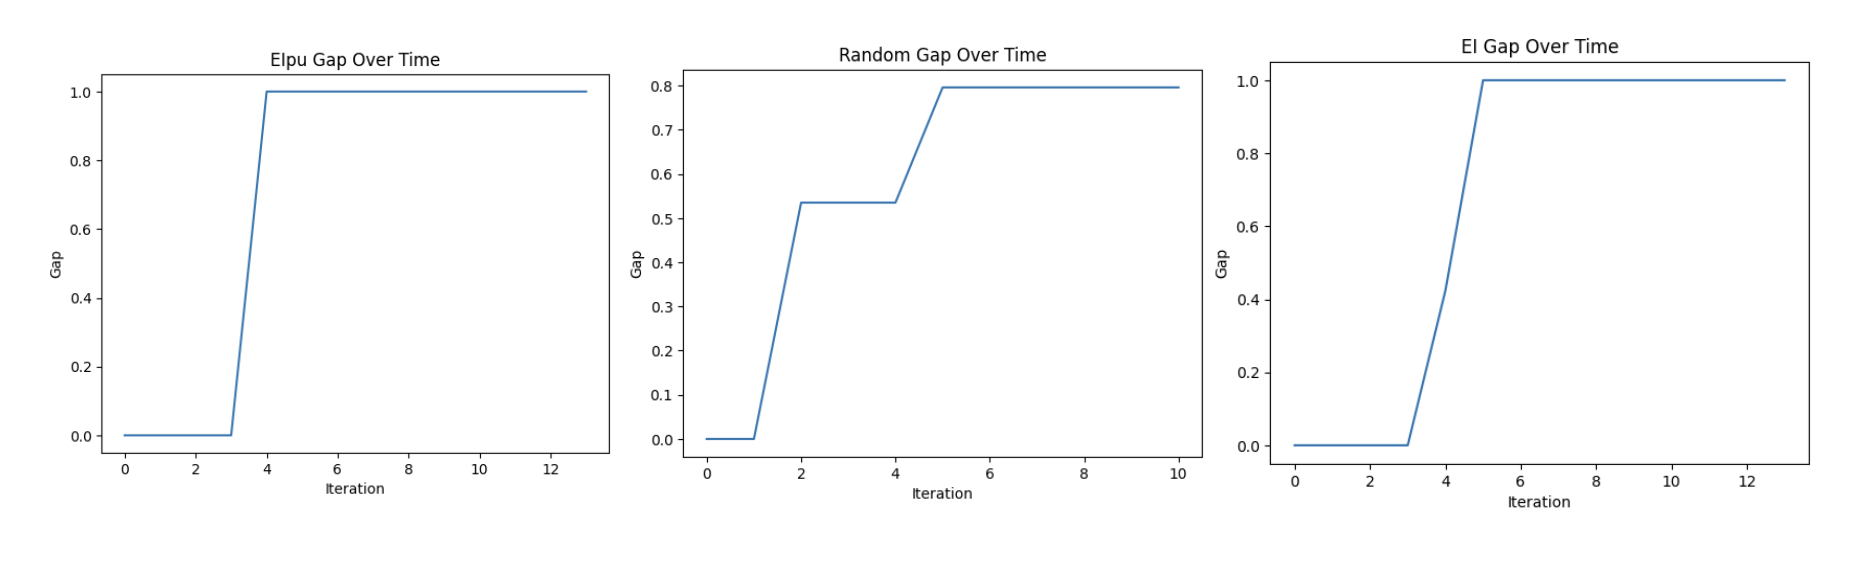
\includegraphics[width=1\linewidth]{graphics/gaps.png}
    \caption{Comparison of gap across optimization techniques}
\end{figure}

% \section{Cost-constrained Bayesian optimization}
% One can think of cost-constrained BO as the following constrained optimization problem:
% \begin{align*}
% \min_{\bfx \in \mathcal{X}} f(\bfx)
% \operatorname{subject \; to} \sum_{\bfx \in \mathcal{X}} c(\bfx)
% \leq \tau.
% \end{align*}
% We assume $f(\bfx)$ outputs not only its value, but also its evaluation cost determined by a 
% black-box cost function $c(\bfx)$. We assume the cost function has the following functional
% form: $c(\bfx) = p(\bfx) + \exp(g(\bfx))$ where $g(\bfx) \sim \mathcal{GP}(m(\bfx), k(\bfx, \bfx')$
% and $p(\bfx) = \sum_{i=0}^d a_ix^i$. That is, the cost consists of an optional deterministic 
% component plus some stochastic perturbation term that is state-independent. Our goal is to
% minimize $f(\bfx)$ subject to the total evaluation cost not exceeding $\tau$. The value of
% $\tau$ is a pre-determined upper bound on the total cost, such as compute time, dollars, or
% cloud-compute resource utilization.
\bibliographystyle{plainnat}
\bibliography{references}
\nocite{*}


%%%%%%%%%%%%%%%%%%%%%%%%%%%%%%%%%%%%%%%%%%%%%%%%%%%%%%%%%%%%

\appendix

\section{Appendix / supplemental material}

\subsection{Expected Improvement}

The expected improvement acquisition function ($EI(x)$) is a common acquisition function for BO. 
\[EI(x) = (f^* - \mu(x))\Phi \left( \frac{f^* - \mu(x)}
{\sigma(x)}\right) + \sigma(x)\phi \left(\frac{f^* - \mu(x)}
{\sigma(x)}\right)\]
where $f^*$ is the best point observed so far and $\mu(x)$, $\sigma(x)$ are the predictive mean and variance at our point $x$. $\Phi$ is the standard normal CDF and $\phi$ is the PDF. The expected improvement acquisition function is powerful as it uses statistics gathered on all prior observations to guide the model where it has the ``best chance'' of finding a value of $f$ which is higher than any previously seen.

\subsection{The Ackley Function}
The Ackley function is expensive to optimize as
\[
f(x) = -a \exp\left(-b \sqrt{\frac{1}{d} \sum_{i=1}^{d} x_i^2}\right) - \exp\left(\frac{1}{d} \sum_{i=1}^{d} \cos(c \, x_i)\right) + a + \exp(1)
\]
where $a = 20$, $b = 0.2$, $c = 2 \pi$, $d = \text{number of dimensions}$.

\subsection{Gap}

\subsection{Markov Decision Process}

%%%%%%%%%%%%%%%%%%%%%%%%%%%%%%%%%%%%%%%%%%%%%%%%%%%%%%%%%%%%

\end{document}